\documentclass[11pt,letterpaper]{article}
\usepackage[letterpaper,margin=0.83in,top=0.78in,bottom=0.75in]{geometry}
\usepackage[T1]{fontenc}
\usepackage{lmodern}
\usepackage{amsmath,booktabs,tabularx,array,tikz}
\usepackage{fancyhdr}
\usepackage[colorlinks=true,linkcolor=teal,urlcolor=teal]{hyperref}

\definecolor{ink}{HTML}{192D3A}
\definecolor{muted}{HTML}{4B6371}
\definecolor{accent}{HTML}{126A70}
\definecolor{control}{HTML}{A7BEC7}
\definecolor{rulecolor}{HTML}{DFE7EA}
\definecolor{wash}{HTML}{EDF5F5}
\hypersetup{pdftitle={ATLAS: Star-field identification and pointing estimation},
    pdfauthor={Skyler Lee}}
\setlength{\parindent}{0pt}
\setlength{\parskip}{5pt}
\setlength{\headheight}{15pt}
\renewcommand{\headrulewidth}{0pt}
\pagestyle{fancy}
\fancyhf{}
\fancyhead[L]{\small\sffamily\color{muted}ATLAS \enspace / \enspace TECHNICAL REPORT}
\fancyfoot[R]{\small\sffamily\color{muted}\thepage}
\color{ink}
\newcommand{\reportsection}[1]{\par\medskip{\large\sffamily\bfseries\color{accent}#1}\par\nobreak\smallskip}
\newcommand{\figurecaption}[1]{\par{\small\color{muted}#1}\par}

% Chart geometry is fixed; bar endpoints use the measured values.
\newcommand{\accuracybars}[5]{%
  \node[anchor=east,font=\small\sffamily] at (-1,#2) {#1};
  \fill[control] (0,{#2+0.04}) rectangle (#3,{#2+0.26});
  \fill[accent] (0,{#2-0.26}) rectangle (#4,{#2-0.04});
  \ifnum#5=1
    \node[anchor=west,font=\scriptsize\sffamily] at (#3,{#2+0.15}) {65.8\%};
    \node[anchor=west,font=\scriptsize\sffamily] at (#4,{#2-0.15}) {86.7\%};
  \fi
}
\newcommand{\runtimebar}[4]{%
  \node[anchor=east,font=\small\sffamily] at (-1,#2) {#1};
  \fill[#4] (0,{#2-0.15}) rectangle (#3,{#2+0.15});
  \node[anchor=west,font=\small\sffamily] at (#3,#2) {#3\,ms};
}

\begin{document}
\thispagestyle{fancy}
{\sffamily\bfseries\fontsize{35}{39}\selectfont ATLAS\par}
{\sffamily\fontsize{20}{24}\selectfont Star-field identification and pointing estimation\par}
\vspace{7pt}
{\sffamily\color{muted}Skyler Lee \enspace$\cdot$\enspace November 2026\par}
\vspace{12pt}
{\color{accent}\rule{\linewidth}{1.2pt}}

\reportsection{Abstract}
ATLAS is a spacecraft star tracker prototype that estimates where a camera is
pointing by matching detected stars to reference fields derived from the Gaia
catalog. In 120 simulated sequences, five-frame ATLAS placed the camera's
pointing direction within \(0.1^\circ\) of ground truth in \textbf{104 of 120
trials (86.7\%)} after 3D refinement. The matched single-frame control reached
\textbf{79 of 120 (65.8\%)} with the same refinement, a gain of
\textbf{20.8 percentage points}. The five-frame pipeline averaged 54.47\,ms
of processing per sequence after star detections were available.

\reportsection{1. Method}
\textbf{Catalog and matching.} ATLAS indexes 1,000 Gaia-derived reference
fields. It ranks candidate fields using anchored triangle fingerprints and
a histogram of pairwise star distances and brightness differences. The two
features supply up to 10 and 30 candidate slots, respectively. A geometric
verification stage checks up to 40 candidates. A 3D fit using matched stars
refines the camera boresight, the direction of its optical axis.

\textbf{Temporal filtering.} The five-frame method registers detected star
positions across frames and keeps tracks present in at least three frames.
Median positions and brightness estimates reduce the influence of transient
false detections and measurement noise before catalog matching.

\reportsection{2. Experimental design}
The temporal benchmark used 120 independent five-frame sequences at unseen
sky directions, with a simulated \(22^\circ\) field of view, random initial roll,
and fixed boresight. The control used the fifth frame of each sequence. Both
conditions used the same catalog, verification budget, and correctness criterion.
Each severity included 40 sequences. The final 30 sequences also contained
a recurring moving false detection.

\smallskip
\begin{tabular*}{\linewidth}{@{\extracolsep{\fill}}lrrrr@{}}
\toprule
\textbf{Severity} & \textbf{Stars removed} & \textbf{False stars} &
  \textbf{Position noise} & \textbf{Brightness noise} \\
\midrule
Moderate & 12\% & 1 & 0.0010 & 0.08 mag \\
Severe   & 27\% & 2 & 0.0025 & 0.18 mag \\
Extreme  & 40\% & 3 & 0.0045 & 0.32 mag \\
\bottomrule
\end{tabular*}
\figurecaption{Table 1. Per-frame perturbations. Noise values are standard deviations in normalized image coordinates and magnitudes.}

\newpage
\reportsection{3. Accuracy under matched conditions}
With 3D refinement, five-frame ATLAS recovered 33 trials missed by the
single-frame control and lost 8 that the control solved. The paired exact
McNemar test gave \(p=1.12\times10^{-4}\). The largest gain was under extreme
corruption, where the number of correct estimates rose from 11 to 28 of 40.
Moderate-case accuracy stayed at 37 of 40.

\smallskip
\begin{center}
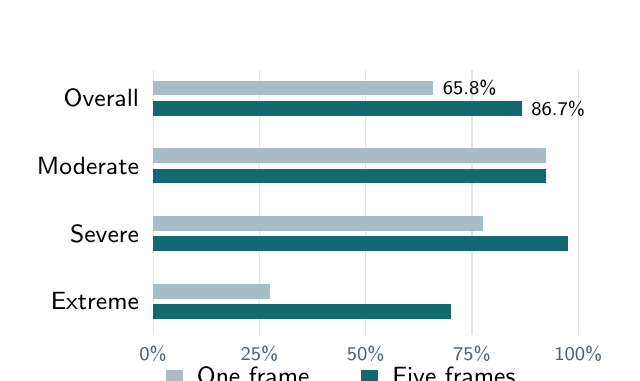
\begin{tikzpicture}[x=0.054cm,y=0.86cm]
  \foreach \tick in {0,25,50,75,100}{
    \draw[rulecolor] (\tick,0.5) -- (\tick,4.42);
    \node[anchor=north,font=\scriptsize\sffamily,text=muted] at (\tick,0.48) {\tick\%};
  }
  \accuracybars{Overall}{4}{65.8333}{86.6667}{1}
  \accuracybars{Moderate}{3}{92.5}{92.5}{0}
  \accuracybars{Severe}{2}{77.5}{97.5}{0}
  \accuracybars{Extreme}{1}{27.5}{70}{0}
  \fill[control] (3,-0.19) rectangle (7,-0.02);
  \node[anchor=west,font=\small\sffamily] at (8,-0.105) {One frame};
  \fill[accent] (49,-0.19) rectangle (53,-0.02);
  \node[anchor=west,font=\small\sffamily] at (54,-0.105) {Five frames};
\end{tikzpicture}
\end{center}
\figurecaption{Figure 1. Share of trials with refined boresight error within \(0.1^\circ\). Overall \(n=120\). Each severity has \(n=40\).}

\reportsection{4. Runtime and comparisons}
ATLAS used 16.01\,ms more compute on average with five frames than with
one. The timed pipeline includes registration, fusion, ranking, and geometric
verification where applicable. Timing starts with detected stars and excludes
image capture, star detection in raw images, and offline catalog preparation.
At 30 frames per second, collecting five frames from the first to the fifth
exposure alone takes about 133\,ms.

\smallskip
\begin{center}
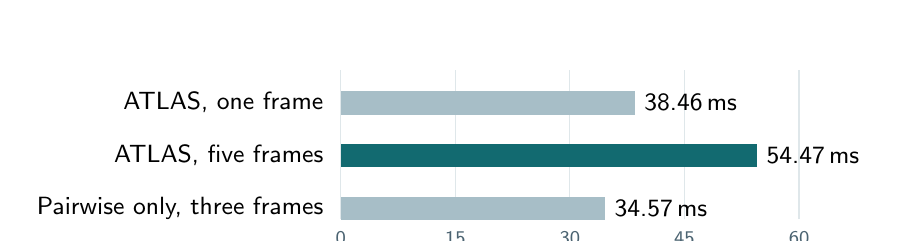
\begin{tikzpicture}[x=0.097cm,y=1.0cm]
  \foreach \tick in {0,15,30,45,60}{
    \draw[rulecolor] (\tick,0.52) -- (\tick,2.42);
    \node[anchor=north,font=\scriptsize\sffamily,text=muted] at (\tick,0.48) {\tick};
  }
  \runtimebar{ATLAS, one frame}{2}{38.46}{control}
  \runtimebar{ATLAS, five frames}{1.33}{54.47}{accent}
  \runtimebar{Pairwise only, three frames}{0.66}{34.57}{control}
\end{tikzpicture}
\end{center}
\figurecaption{Figure 2. Mean measured processing time per solution in milliseconds. The three-frame pairwise result comes from the temporal ablation.}

Before 3D refinement, five-frame ATLAS reached 91 of 120 correct estimates,
versus 64 of 120 for one frame. The three-frame pairwise-only variant reached
88 of 120 in 34.57\,ms. With five frames, pairwise-only reached 90 of 120 in
48.59\,ms. The one-trial difference between five-frame pairwise-only and
five-frame ATLAS provides limited evidence of a benefit from the triangle features.

\newpage
\reportsection{5. Supporting benchmarks}
\smallskip
\begin{tabularx}{\linewidth}{@{}>{\raggedright\arraybackslash}Xrrrr@{}}
\toprule
& \multicolumn{2}{c}{\textbf{One frame}} & \multicolumn{2}{c}{\textbf{Five frames}} \\
\cmidrule(lr){2-3}\cmidrule(l){4-5}
\textbf{Method} & \textbf{Correct} & \textbf{Mean ms} & \textbf{Correct} & \textbf{Mean ms}\\
\midrule
ATLAS triangle and pairwise brightness & 79/120 & 38.46 & 104/120 & 54.47 \\
Best-anchor and pairwise features & 76/120 & 33.82 & 101/120 & 50.06 \\
Six-anchor assignment and pairwise features & 78/120 & 35.14 & 103/120 & 51.39 \\
\bottomrule
\end{tabularx}
\figurecaption{Table 2. Refined pointing accuracy within \(0.1^\circ\) and mean processing time in the matched temporal benchmark.}

\medskip
\textbf{Brightness ablation.}
In a separate 120-image experiment, adding a histogram that combines
pairwise distance and brightness difference raised refined single-frame
accuracy from 80/120 to 89/120. Adding per-triangle brightness as well
left the refined total at 89/120. Multiple feature weights were explored,
so the gain remains exploratory.

\textbf{Historical Tetra3 comparison.}
On 90 separate simulated observations, an earlier ATLAS hybrid averaged
34.5\,ms versus 160.6\,ms for ESA Tetra3. Under the reported approximate
boresight comparison, the hybrid scored 49/90 and Tetra3 scored 51/90.
The solvers used different reference catalogs and estimation procedures.
This comparison provides runtime context for the earlier hybrid.

\reportsection{6. Limitations}
The benchmark used simulated detections generated from Gaia data. The
1,000-field catalog limits the coverage evaluated. The temporal test held
boresight fixed while varying roll, so it leaves performance during
yaw and pitch maneuvers open. Persistent artifacts were only partly
modeled. The accuracy figures concern boresight pointing. Full three-axis
attitude accuracy, performance on real imagery, and onboard processor
timings remain unmeasured.

\reportsection{7. Interpretation}
The clearest result is the 25-trial net gain from five-frame filtering in
the matched 120-sequence benchmark. The gain was largest when the camera
observations contained substantial star loss and false detections. The
close five-frame pairwise-only result leaves the contribution of the
triangle fingerprint uncertain.

\reportsection{Benchmark records}
{\small
\href{run:atlas_temporal_report.md}{Temporal benchmark report}
\enspace$\cdot$\enspace
\href{run:../results/atlas_temporal_results.csv}{Temporal trial data}
\enspace$\cdot$\enspace
\href{run:../results/atlas_temporal_ablation_results.csv}{Temporal ablation data}

\href{run:atlas_relative_brightness_report.md}{Relative brightness ablation}
\enspace$\cdot$\enspace
\href{run:lightweight_anchor_optimization_report.md}{Earlier hybrid and Tetra3 benchmark}
\par}
\end{document}
